\documentclass[a4paper,12pt]{article}

% --- Pacchetti Fondamentali ---
\usepackage[utf8]{inputenc} % Codifica caratteri
\usepackage[T1]{fontenc}    % Codifica font
\usepackage[italian]{babel} % Lingua italiana
\usepackage{geometry}       % Gestione margini
\usepackage{csquotes}      % Raccomandato da biblatex con babel/polyglossia
\usepackage{parskip}        % Gestione spazi tra paragrafi

\geometry{a4paper, margin=2.5cm}

% --- Pacchetti Matematica e Fisica ---
\usepackage{amsmath, amssymb} % Simboli matematici
\usepackage{siunitx}          % Gestione unità di misura e numeri (FONDAMENTALE)
\sisetup{
    output-decimal-marker = {.}, % Punto come separatore decimale
    separate-uncertainty = true, % Scrive errori come (Valore +/- Errore)
    per-mode = power,            % Usa / per le unità (m/s)
    inter-unit-product = \ensuremath{\cdot} % Per scrivere le unità con il punto (N·m)
}

% --- Pacchetti Immagini e Tabelle ---
\usepackage{graphicx} % Per inserire PNG/JPG
\usepackage{float}    % Per forzare la posizione delle immagini (H)
\usepackage{booktabs} % Per tabelle professionali (\toprule, \midrule)
\usepackage{caption}  % Per personalizzare le didascalie
\usepackage{subcaption}
\usepackage[font=small, labelfont=bf]{caption}
\usepackage[font=small, labelfont=bf]{subcaption}

% --- Dati Intestazione ---
\title{\textbf{Risposta spettroscopica e dispersione elettromagnetica}}
\author{Filippo Audisio, Cataldo Insalaco, Telemaco Pezzoni}
\date{\today}

\begin{document}

\maketitle

% -------------------------------------------------------------------

\section{Obiettivo dell'esperienza}
L'obiettivo dell'esperienza è studiare tecniche spettroscopiche mirate a conoscere la risposta elettromagnetica di materiali massivi su ampio intervallo spettrale, così da poter determinare la loro relazione di dispersione. In particolare si vuole:
\begin{itemize}
    \item Determinare lo spettro di Trasmittanza di vetro amorfo in $SiO_2$ e di Riflettanza di $Si$ cristallino.
    \item Stimare la dispersione dell'indice di rifrazione per il silicio cristallino.
    \item Determinare gli spettri di Trasmittanza e Riflettanza per un materiale incognito.
\end{itemize}

% -------------------------------------------------------------------
\section{Materiali e Metodi}

\subsection{Dotazione sperimentale}
\begin{itemize}
    \item Sorgente a lampada alogena $QTH_{10}$.
    \item Lente accoppiata alla lampada.
    \item Tripletto di lenti per la focalizzazione.
    \item Reticolo diffrattivo 1D a $1000$ \unit{linee/mm}.
    \item Goniometro monocromatore a dispersione.
    \item Fotodiodo in $Si$ polarizzato in inversa con carico $10/47$ \unit{k\Omega}.
    \item Laser di varie lunghezze d'onda: $635.9$\unit{nm}, $532$\unit{nm}, $449.1$\unit{nm}, $406.5$\unit{nm},
    \item Multimetro
    \item Campioni: vetro amorfo in $SiO_2$ spesso $1$\unit{mm}, $Si$ cristallino spesso $0.5$\unit{mm}, materiale incognito n°7.
\end{itemize}

\subsection{Procedura sperimentale}
\begin{enumerate}
    \item \textbf{Allineamento e Calibrazione}: L'intero apparato è stato allineato utilizzando le sorgenti laser, massimizzando l'intensità del segnale rivelato dal fotodiodo con il carico di $10$ \unit{k\Omega} in assenza del reticolo di diffrazione. Successivamente, a seguito dell'inserimento del reticolo nel sistema, si è verificata la calibrazione accertandosi che le lunghezze d'onda ricavate dalle letture del goniometro coincidessero con i valori nominali dei laser.
    \item \textbf{Misure di Trasmittanza}: Nel setup è stata inserita la lampada alogena con la relativa lente di accoppiamento e, mantenendo la resistenza da $10$ \unit{k\Omega}, si è acquisito il primo spettro di baseline. In seguito il campione di vetro amorfo è stato interposto tra sorgente e reticolo di diffrazione per misurarne lo spettro di trasmittanza, normalizzato rispetto alla baseline ricavata in precedenza. Infine la medesima procedura è stata effettuata sul campione incognito.
    \item \textbf{Misure di Riflettanza}: La resistenza di carico nel fotodiodo è stata sostituita con una da $47$ \unit{k\Omega}, così da amplificare il segnale rivelato, procedendo quindi alla misurazione di un secondo spettro di baseline. Dopodiché il sistema è stato portato in configurazione di riflessione per acquisisre gli spettri di Riflettanza del campione di silicio e, in seguito, del campione incognito.     
\end{enumerate}

\begin{figure}[H]
     \centering
     \begin{subfigure}[b]{0.45\textwidth}
         \centering
         
\includegraphics[width=\textwidth]{configurazione_trasmissione.png}
         \subcaption{Configurazione di trasmissione.}
         \label{fig:1a}
     \end{subfigure}
     \begin{subfigure}[b]{0.45\textwidth}
         \centering
         
\includegraphics[width=\textwidth]{configurazione_riflessione.png}
         \subcaption{Configurazione di riflessione.}
         \label{fig:1b}
     \end{subfigure}
\end{figure}
% -------------------------------------------------------------------
\section{Dati sperimentali e Analisi}
\subsection{Spettri}
\subsubsection{Baseline}

\begin{figure}[H]
     \centering
     \begin{subfigure}[b]{0.45\textwidth}
         \centering
         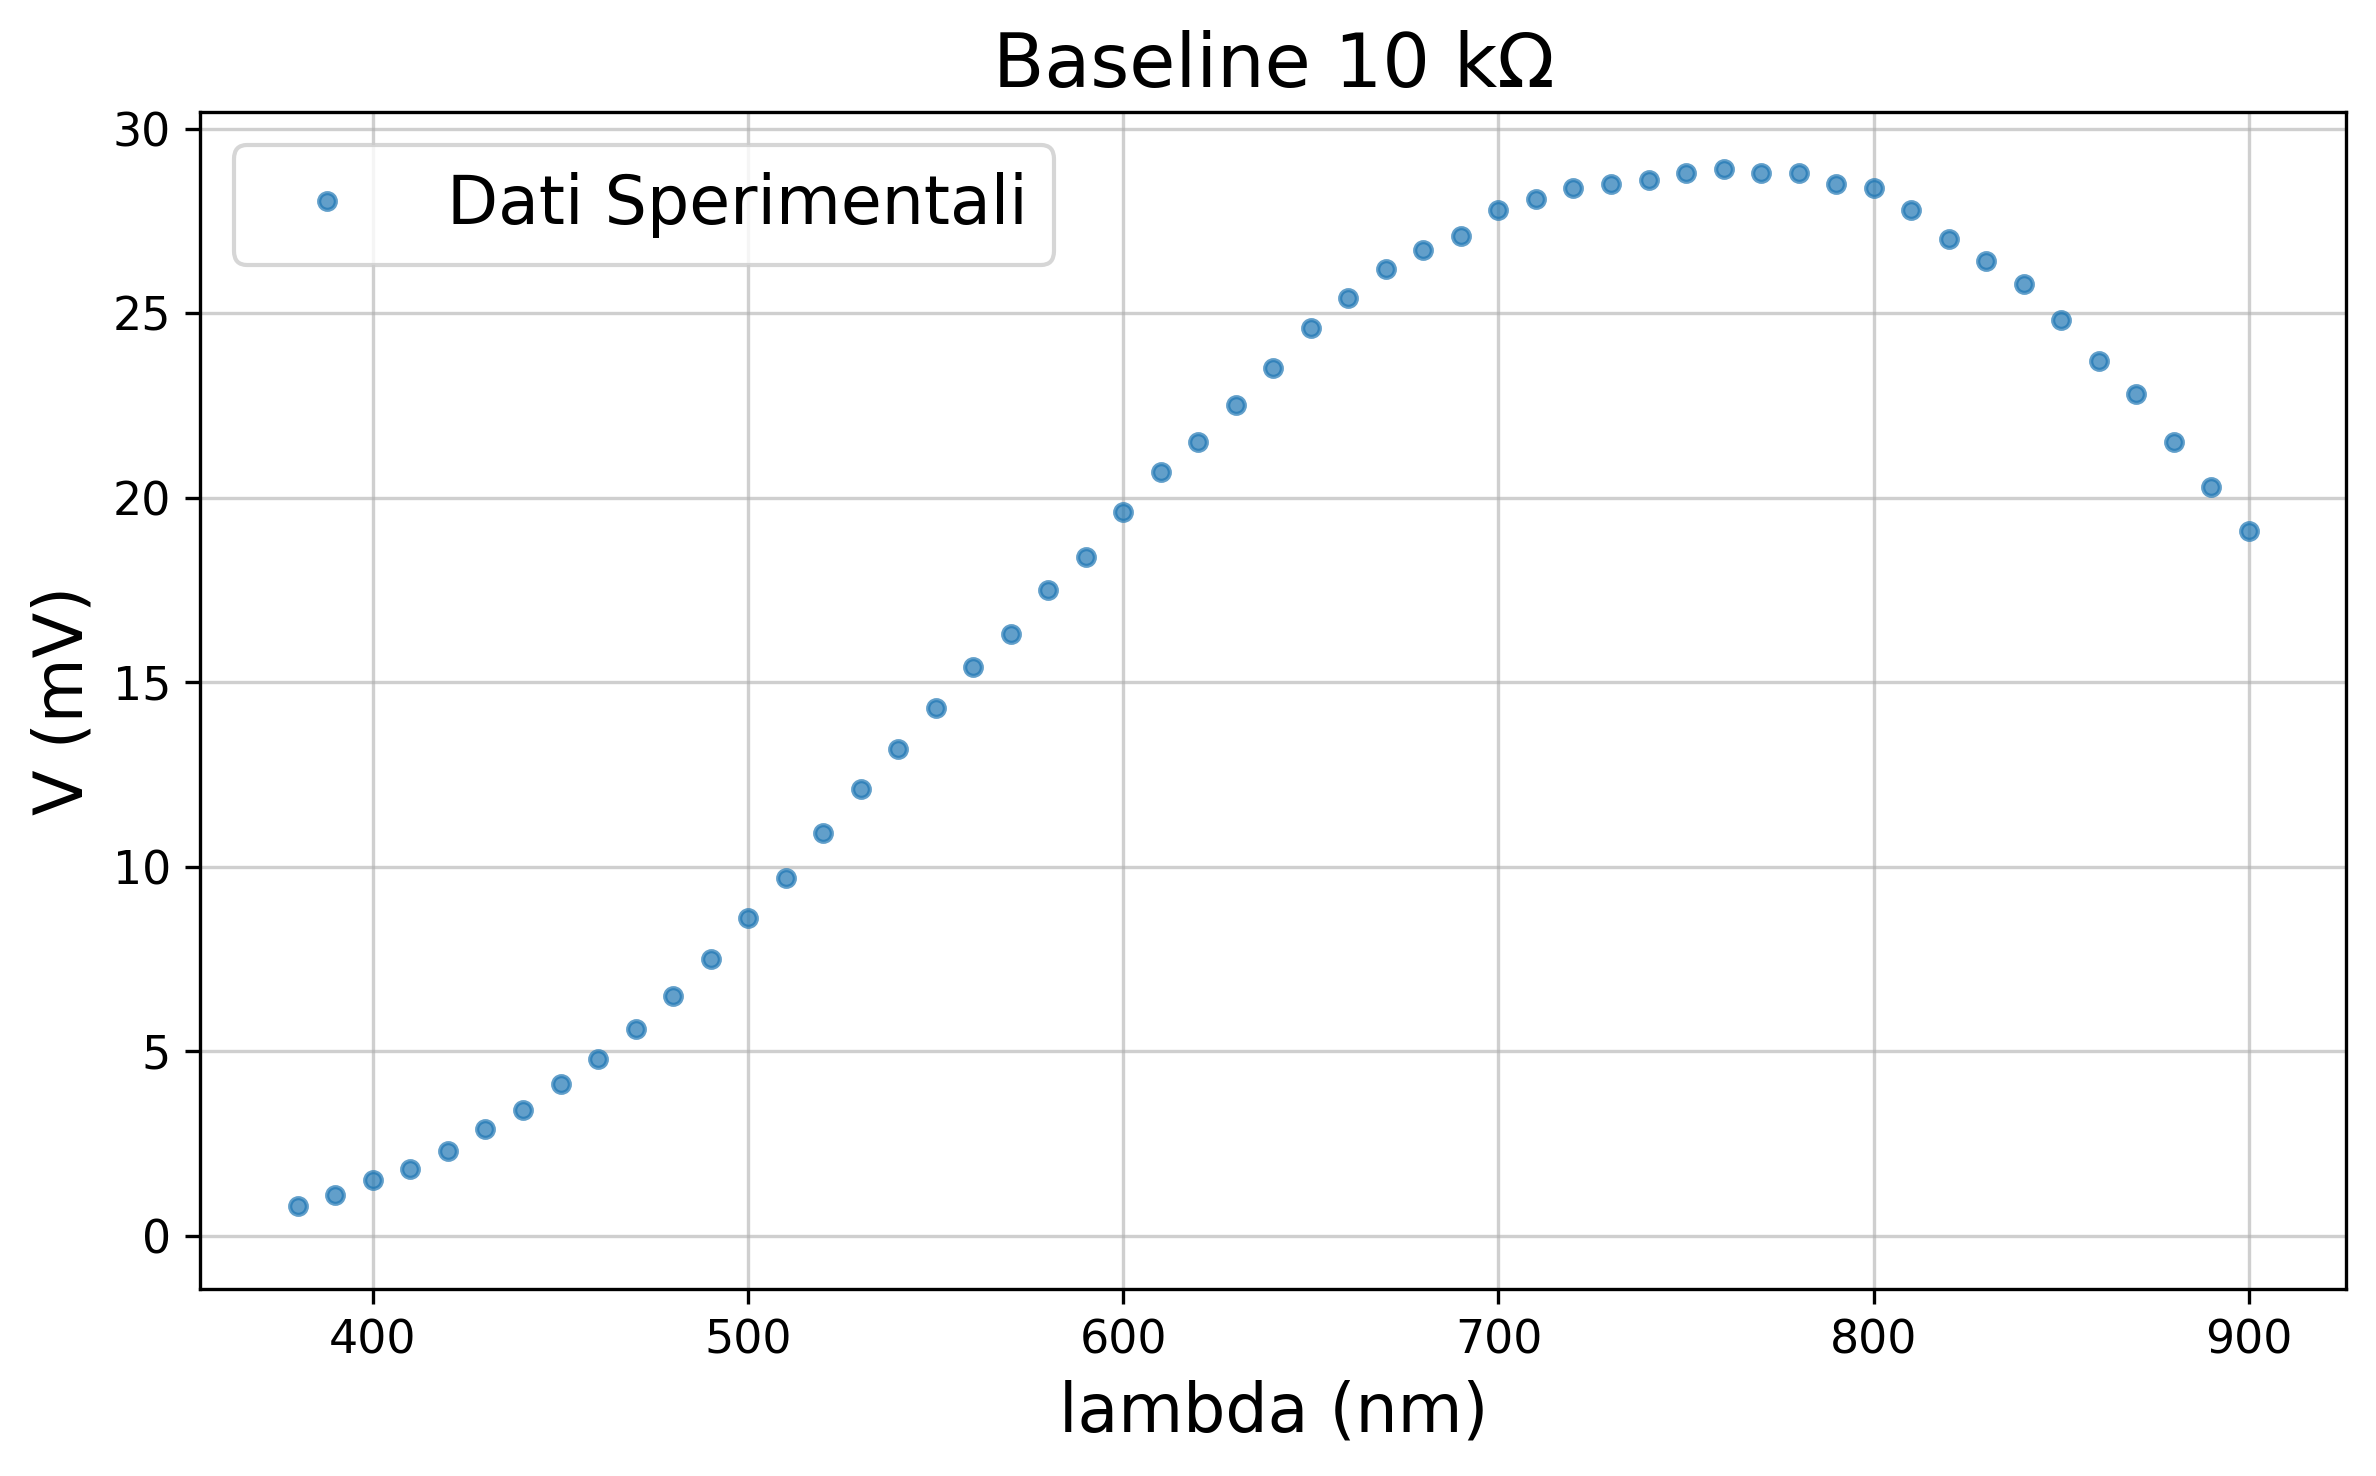
\includegraphics[width=\textwidth]{Dati_Baseline 10 kΩ.png}
         \label{fig:2a}
     \end{subfigure}
     \begin{subfigure}[b]{0.45\textwidth}
         \centering
         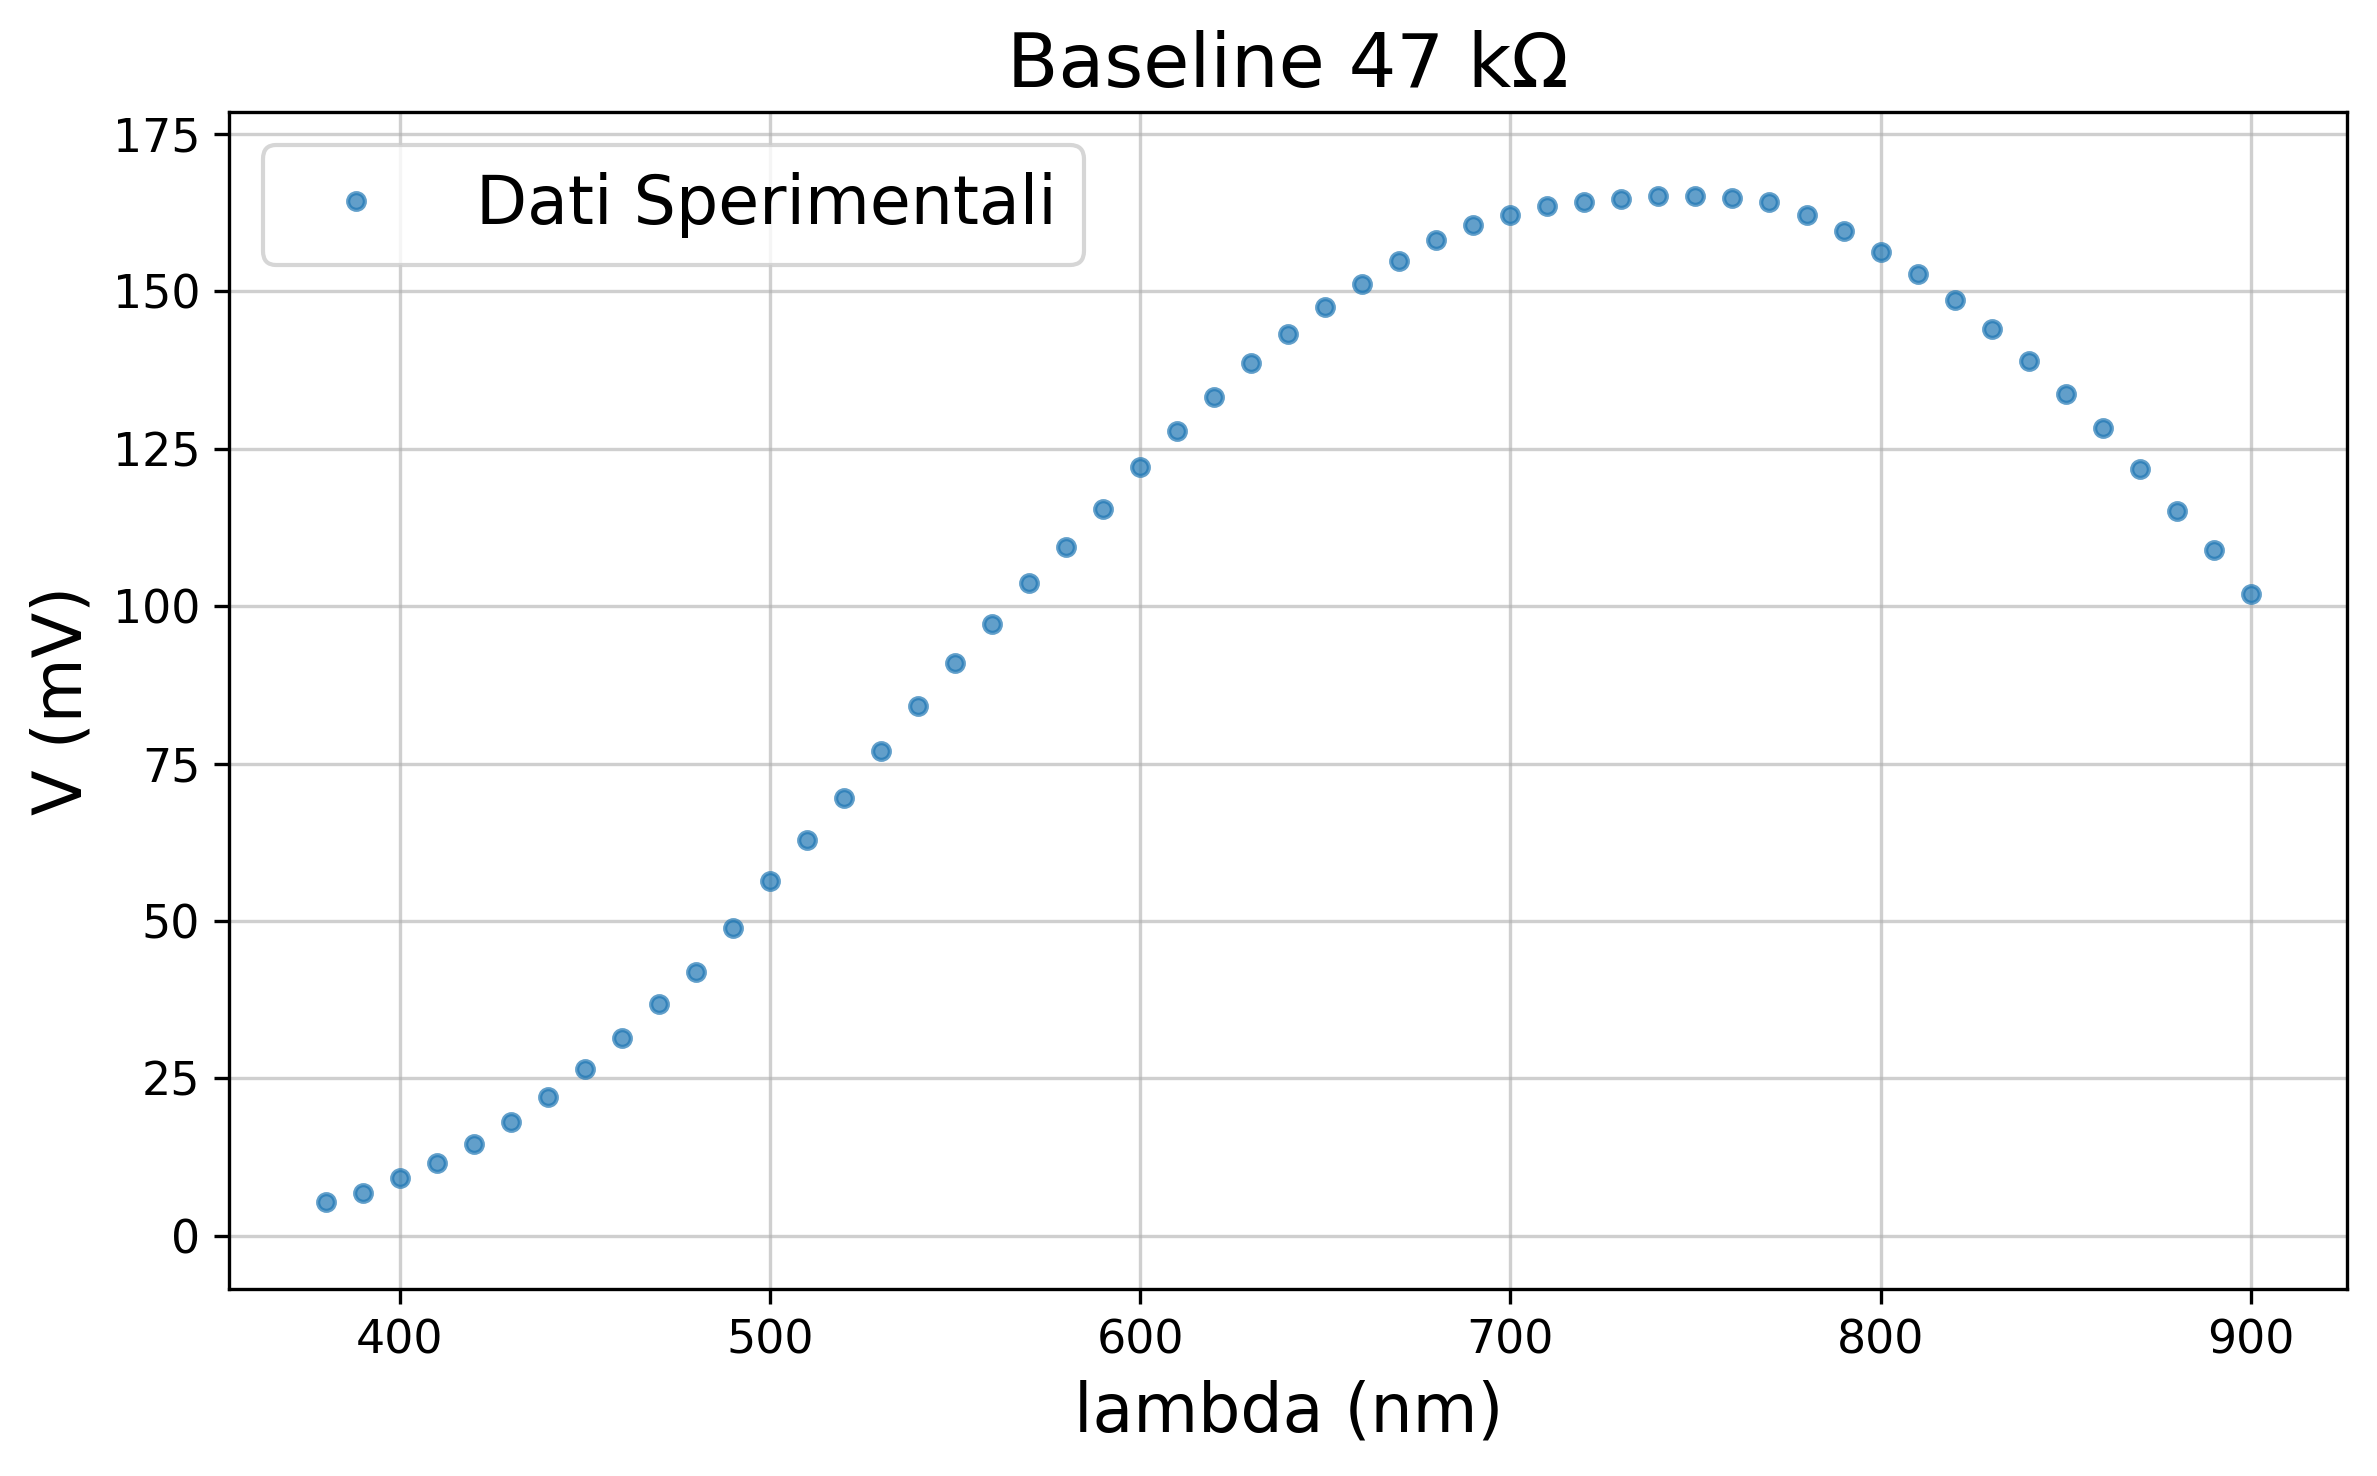
\includegraphics[width=\textwidth]{Dati_Baseline 47 kΩ.png}
         \label{fig:2b}
     \end{subfigure}
\end{figure}

\subsubsection{Vetro amorfo}
\begin{figure}[H]
    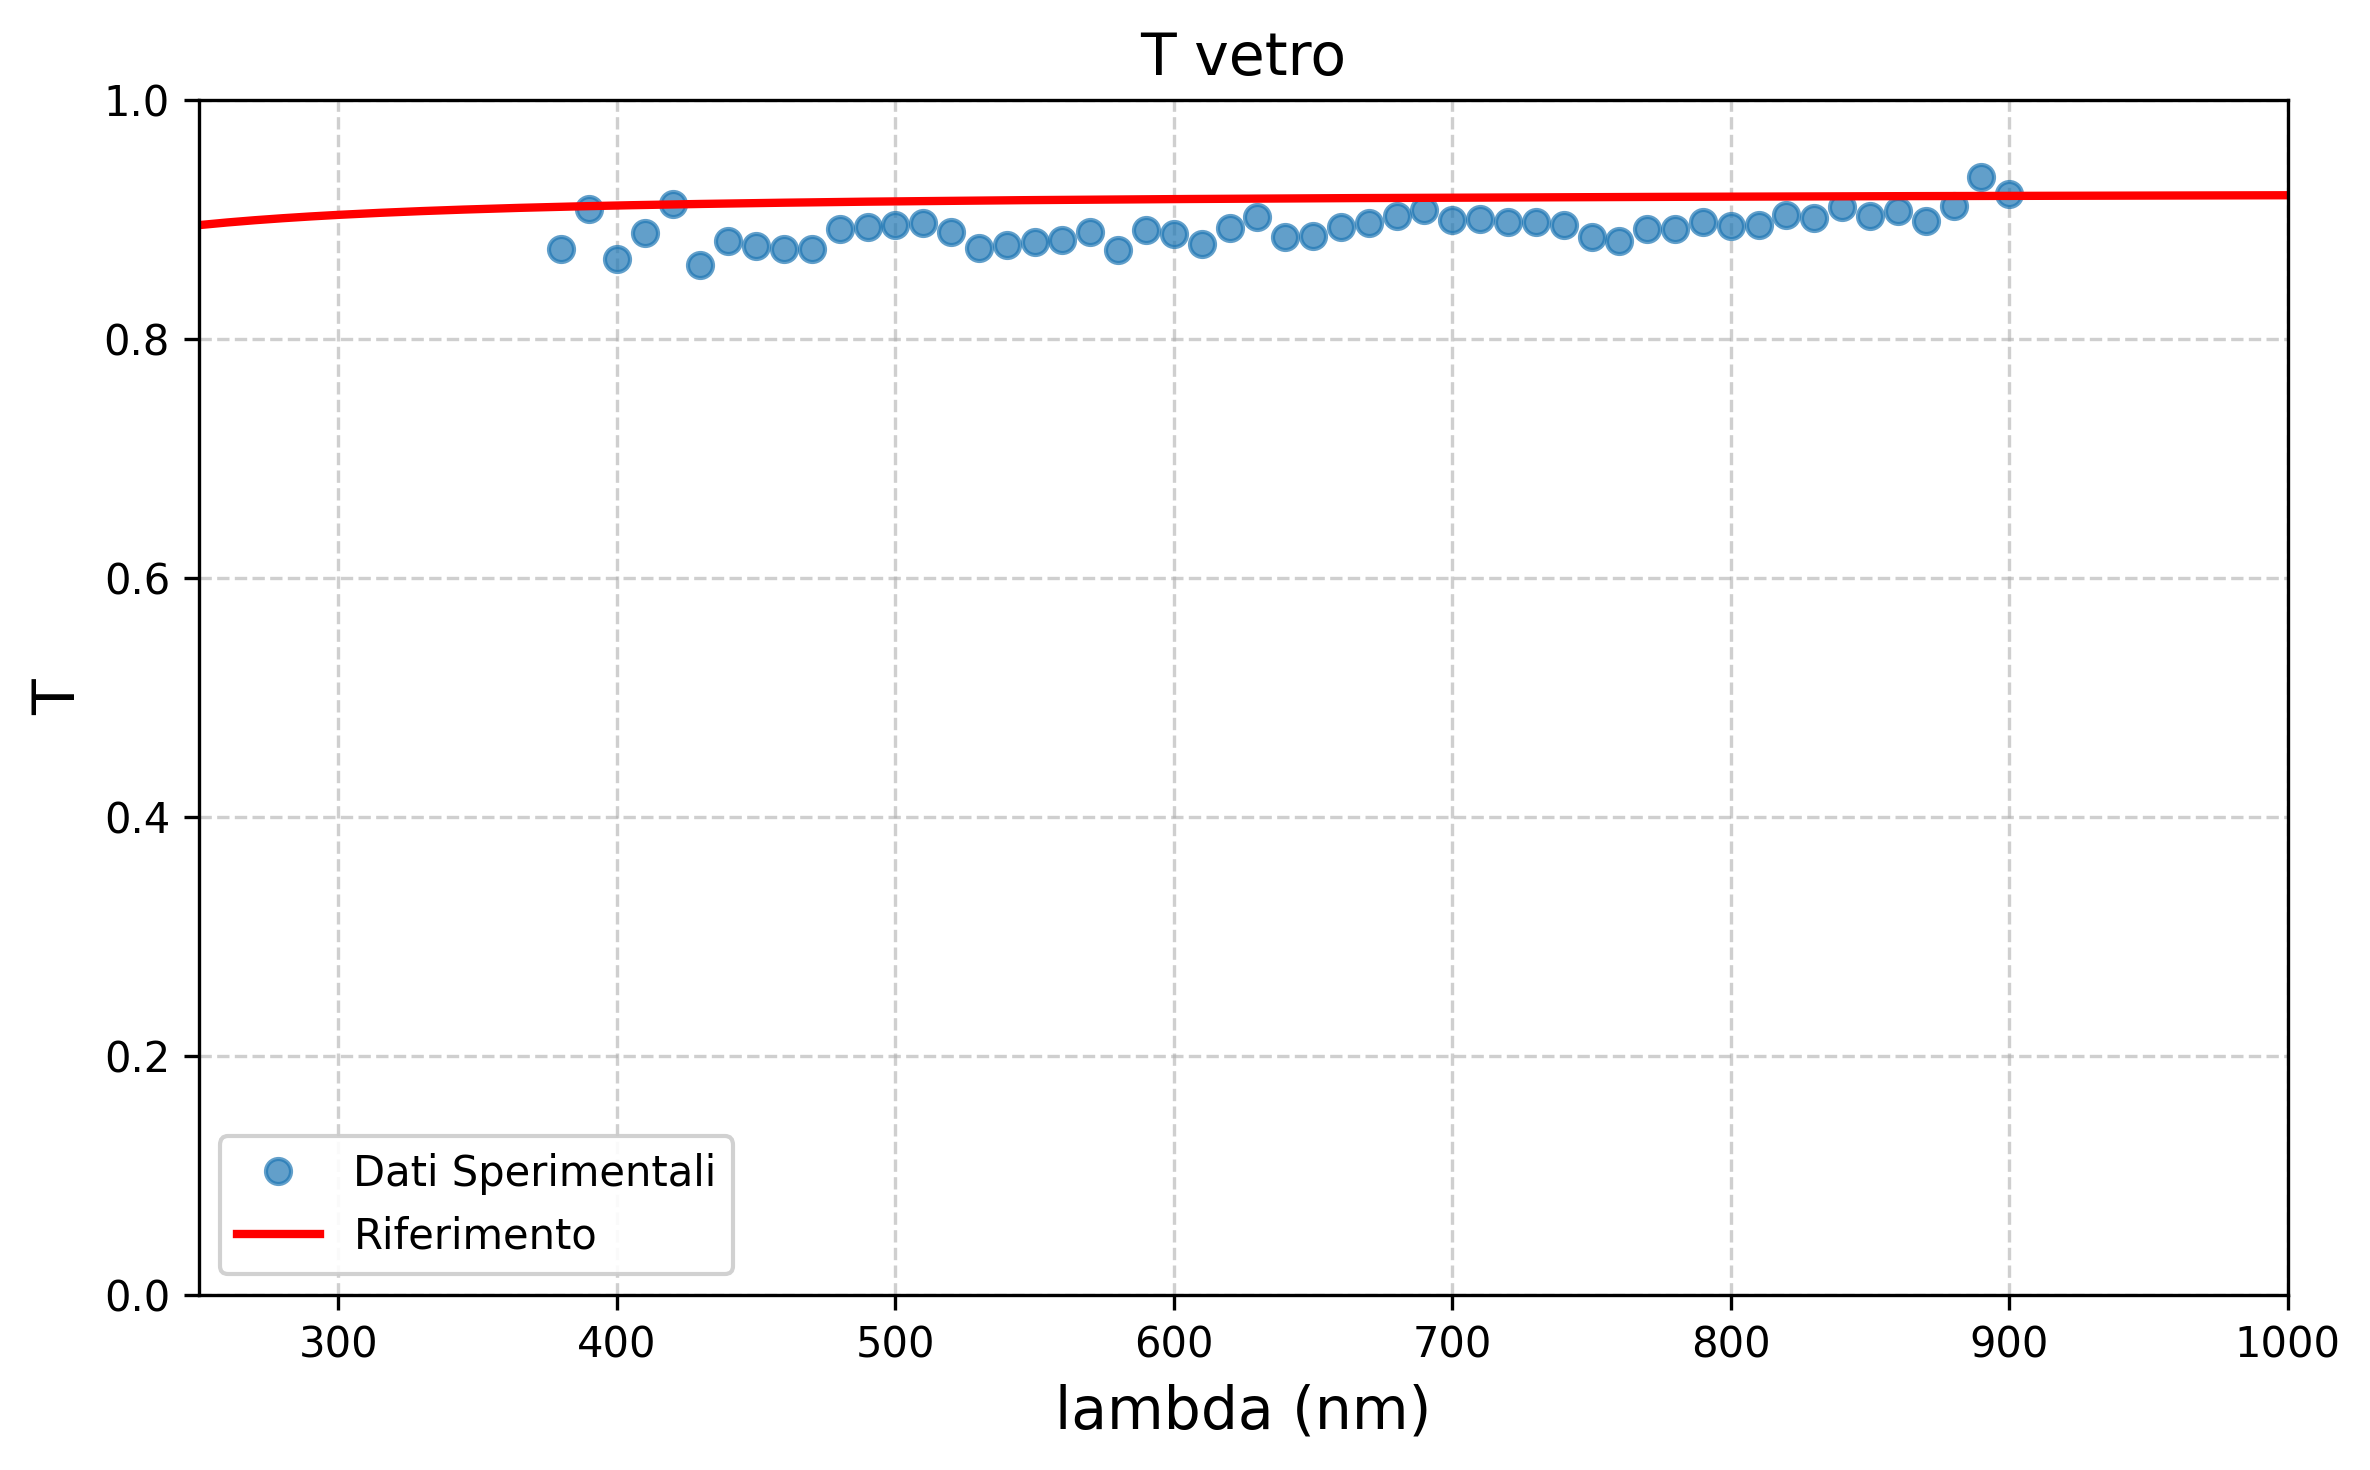
\includegraphics[width=\textwidth]{Confronto_T vetro.png}
    \caption{Spettro di trasmittanza del vetro amorfo confrontato con il riferimento.}
\end{figure}

\subsubsection{Silicio}
\begin{figure}[H]
    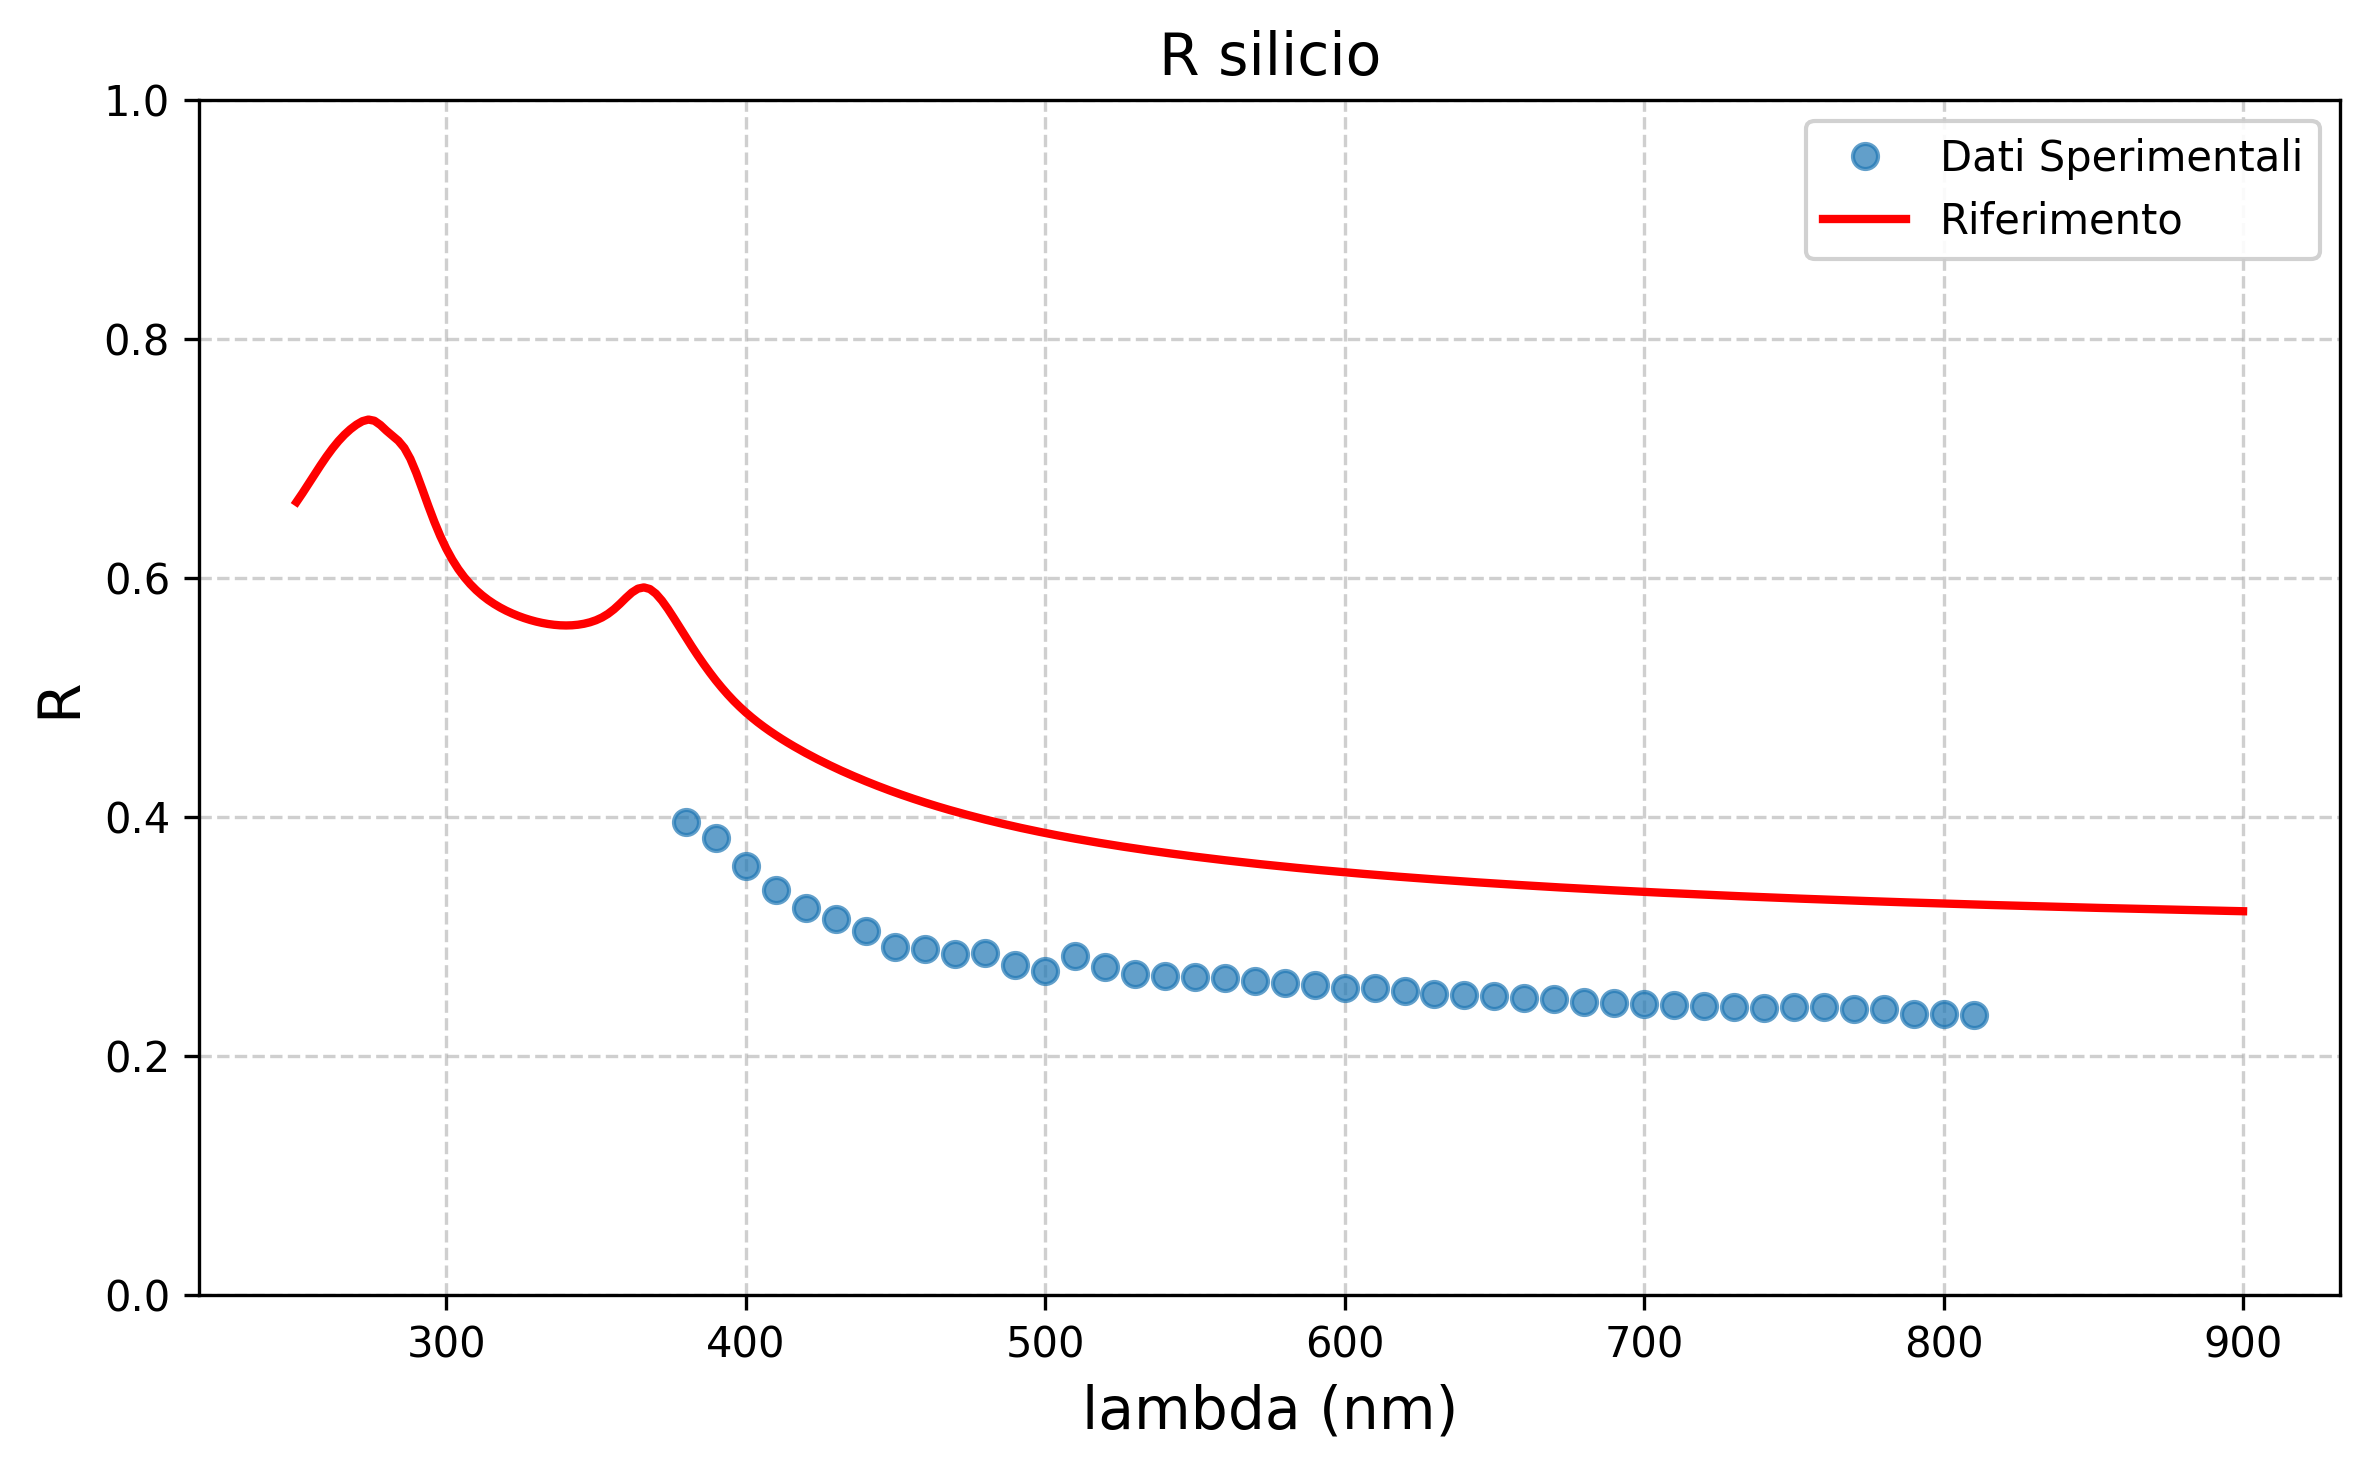
\includegraphics[width=\textwidth]{Confronto_R silicio.png}
    \caption{Spettro di riflettanza del silicio confrontato con il riferimento.}
\end{figure}

\subsection{Dispersione indice di rifrazione}
Dai dati di riflettanza del silicio cristallino si ricava l'indice di rifrazione corrispondente a ciascuna lunghezza d'onda sfruttando la relazione:
\begin{equation}
    n = \frac{1+\sqrt{R}}{1-\sqrt{R}}
\end{equation}
Dopodiché i valori ottenuti sono stati fittati con il modello di Cauchy:
\begin{equation}
    n(\lambda) = A + \frac{B}{\lambda^2} + \frac{C}{\lambda^4}
\end{equation}
\begin{figure}[H]
    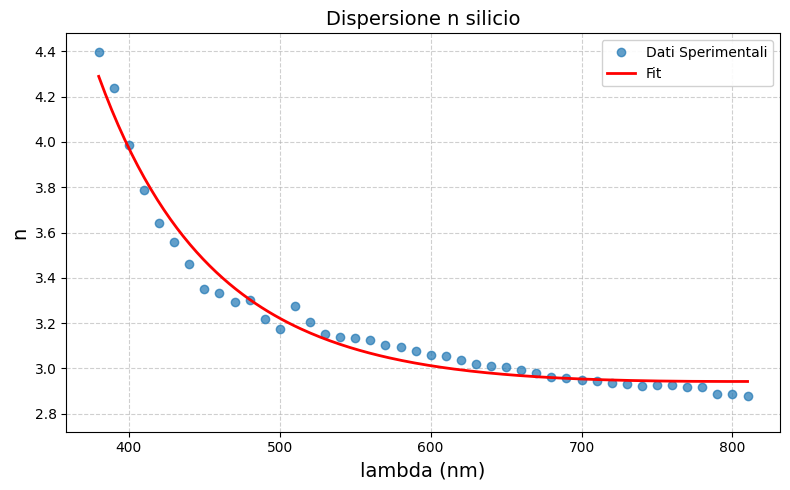
\includegraphics[width=\textwidth]{Fit_Cauchy_n.png}
    \caption{Dispersione dell'indice di rifrazione del Silicio con fit di Cauchy.}
\end{figure}

\begin{table}[H]
    \centering
    \begin{tabular}{
        l
        S[table-format=-2.4e2]  
        S[table-format=2.4e2]
    }
        \toprule
        {Parametro} & {Valore} & {$\sigma$} \\
        \midrule
        $A$ & 3.06 & 0.05 \\
        $B$ [\unit{\mu m^2}] & -1.46e-1 & 0.31e-1 \\
        $C$ [\unit{\mu m^4}] & 4.68e-2 & 0.39e-2 \\
        \bottomrule
    \end{tabular}
    \label{tab:Calibrazione}
\end{table}

\subsection{Materiale Incognito}
\begin{figure}[H]
     \centering
     \begin{subfigure}[b]{0.45\textwidth}
         \centering
         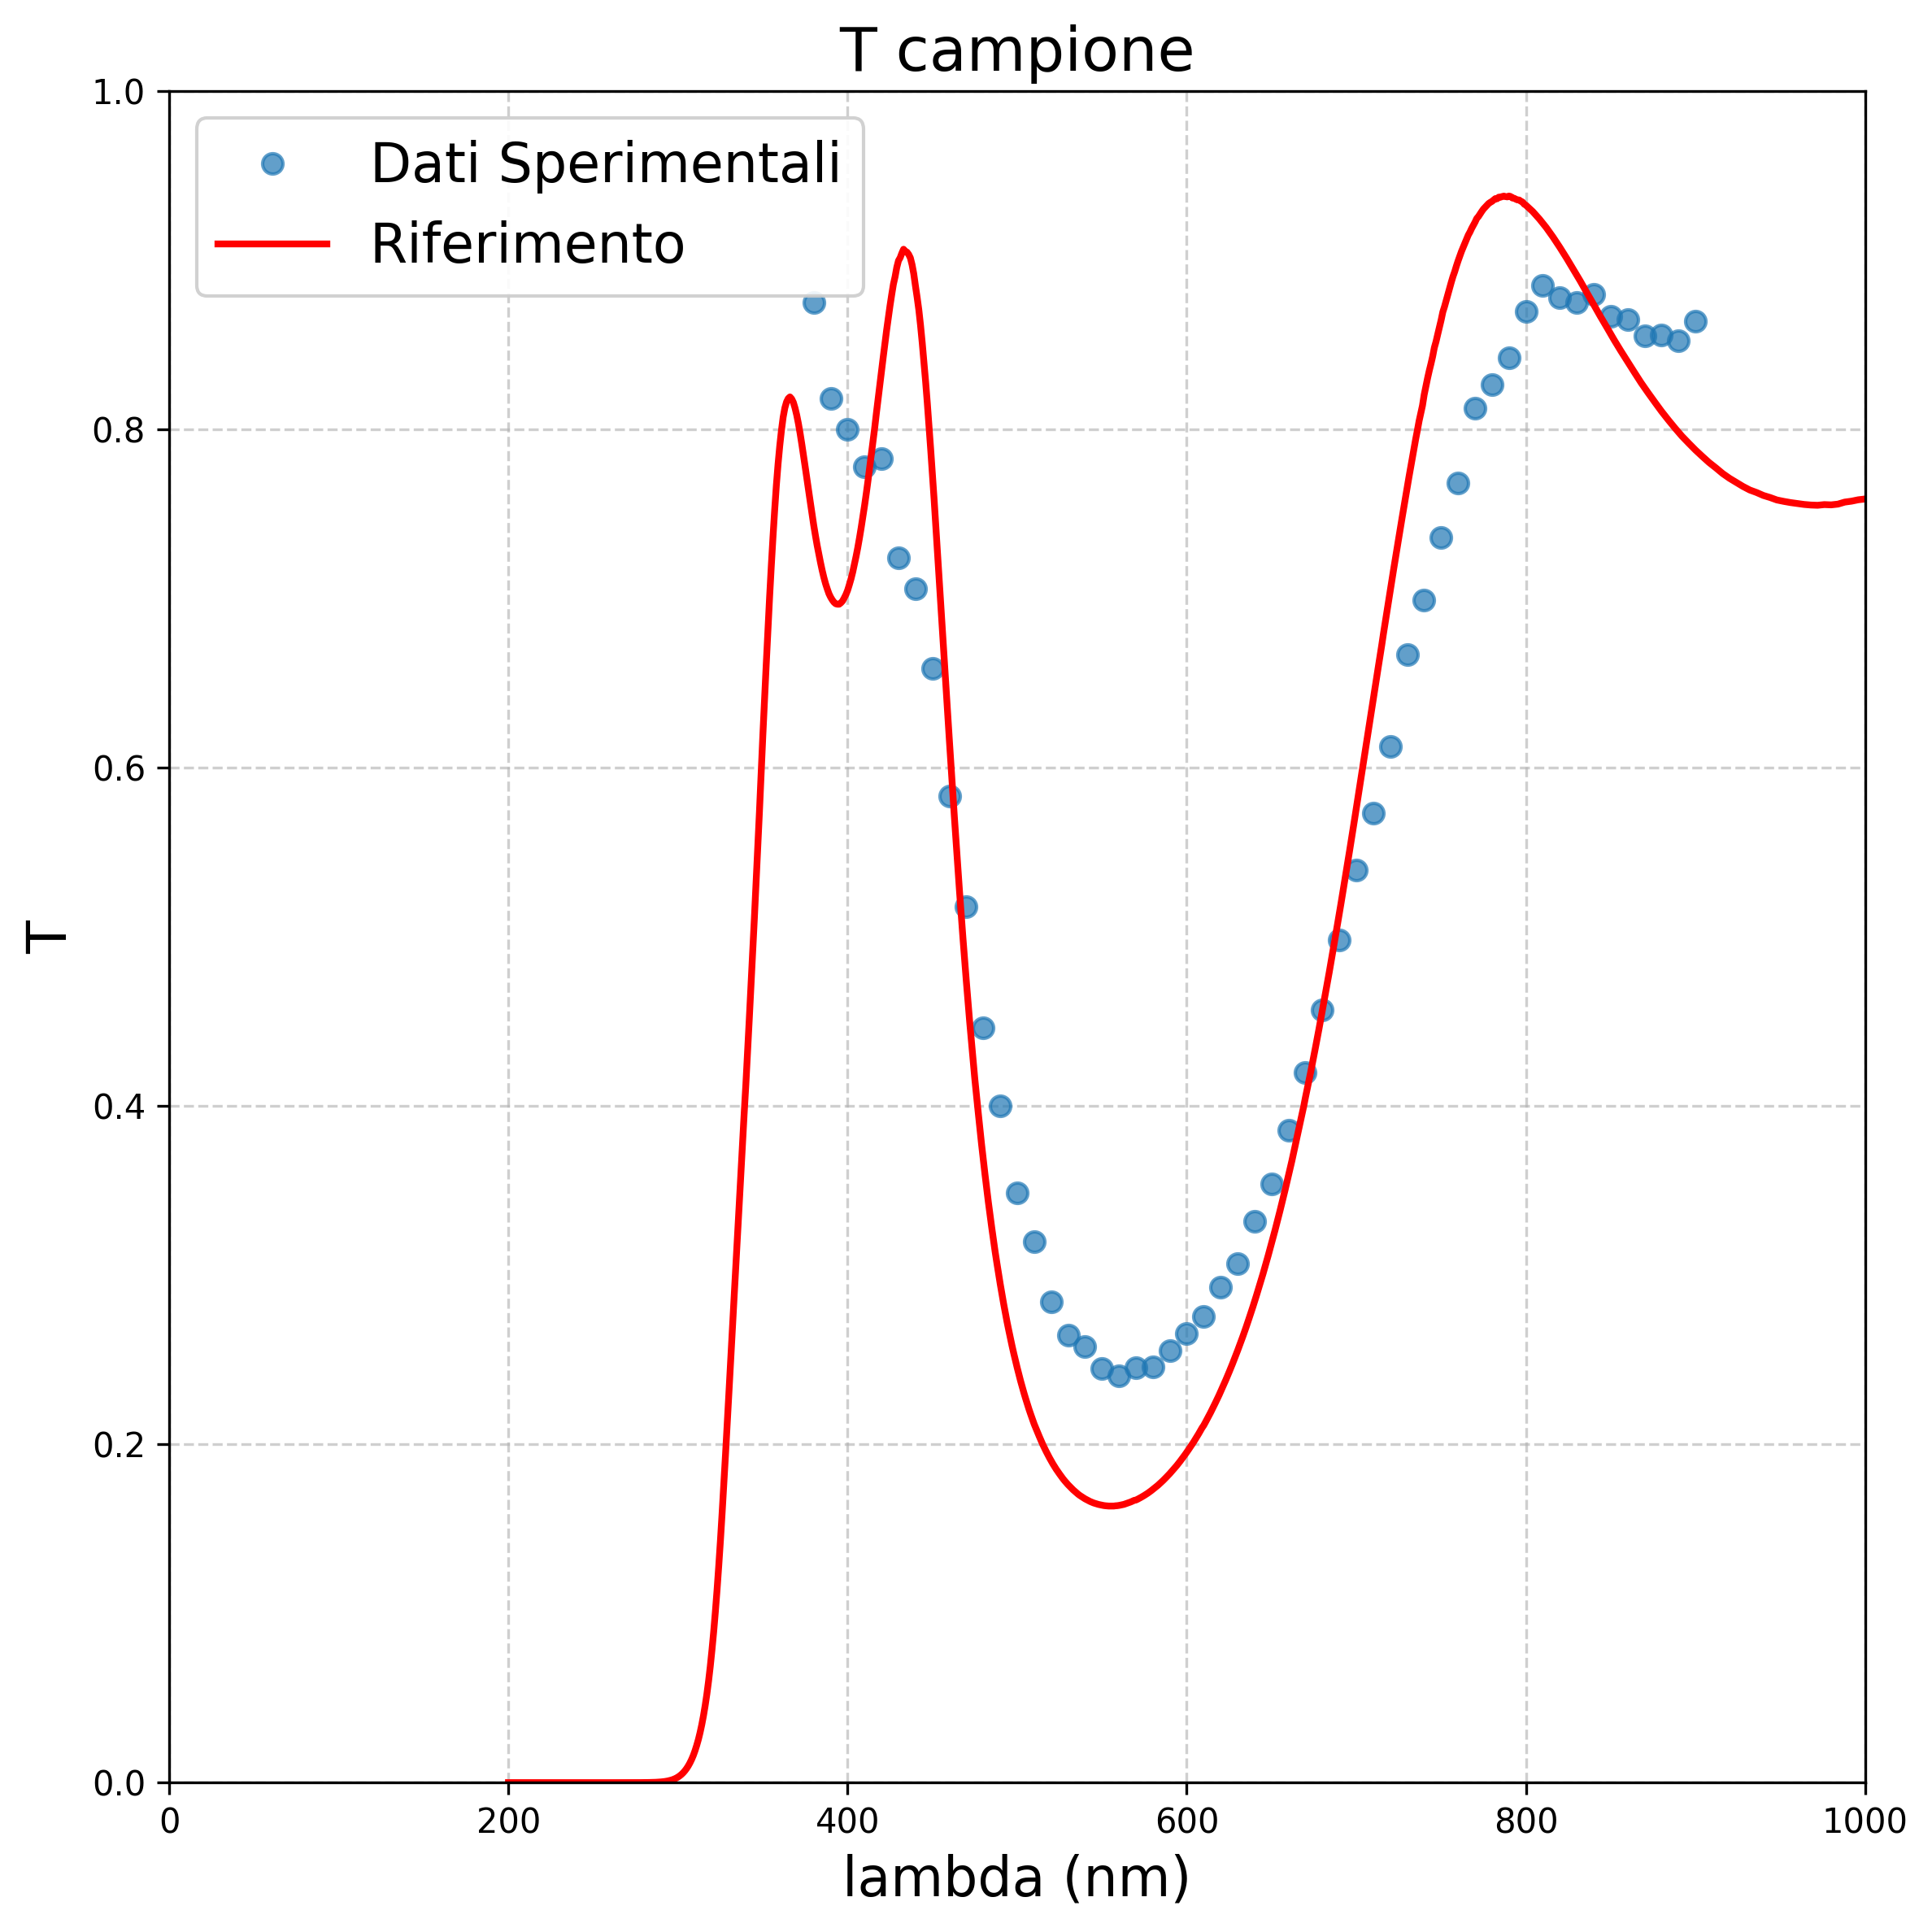
\includegraphics[width=\textwidth]{Confronto_T campione.png}
         \subcaption{Spettro di trasmittanza campione n°7}
     \end{subfigure}
     \begin{subfigure}[b]{0.45\textwidth}
         \centering
         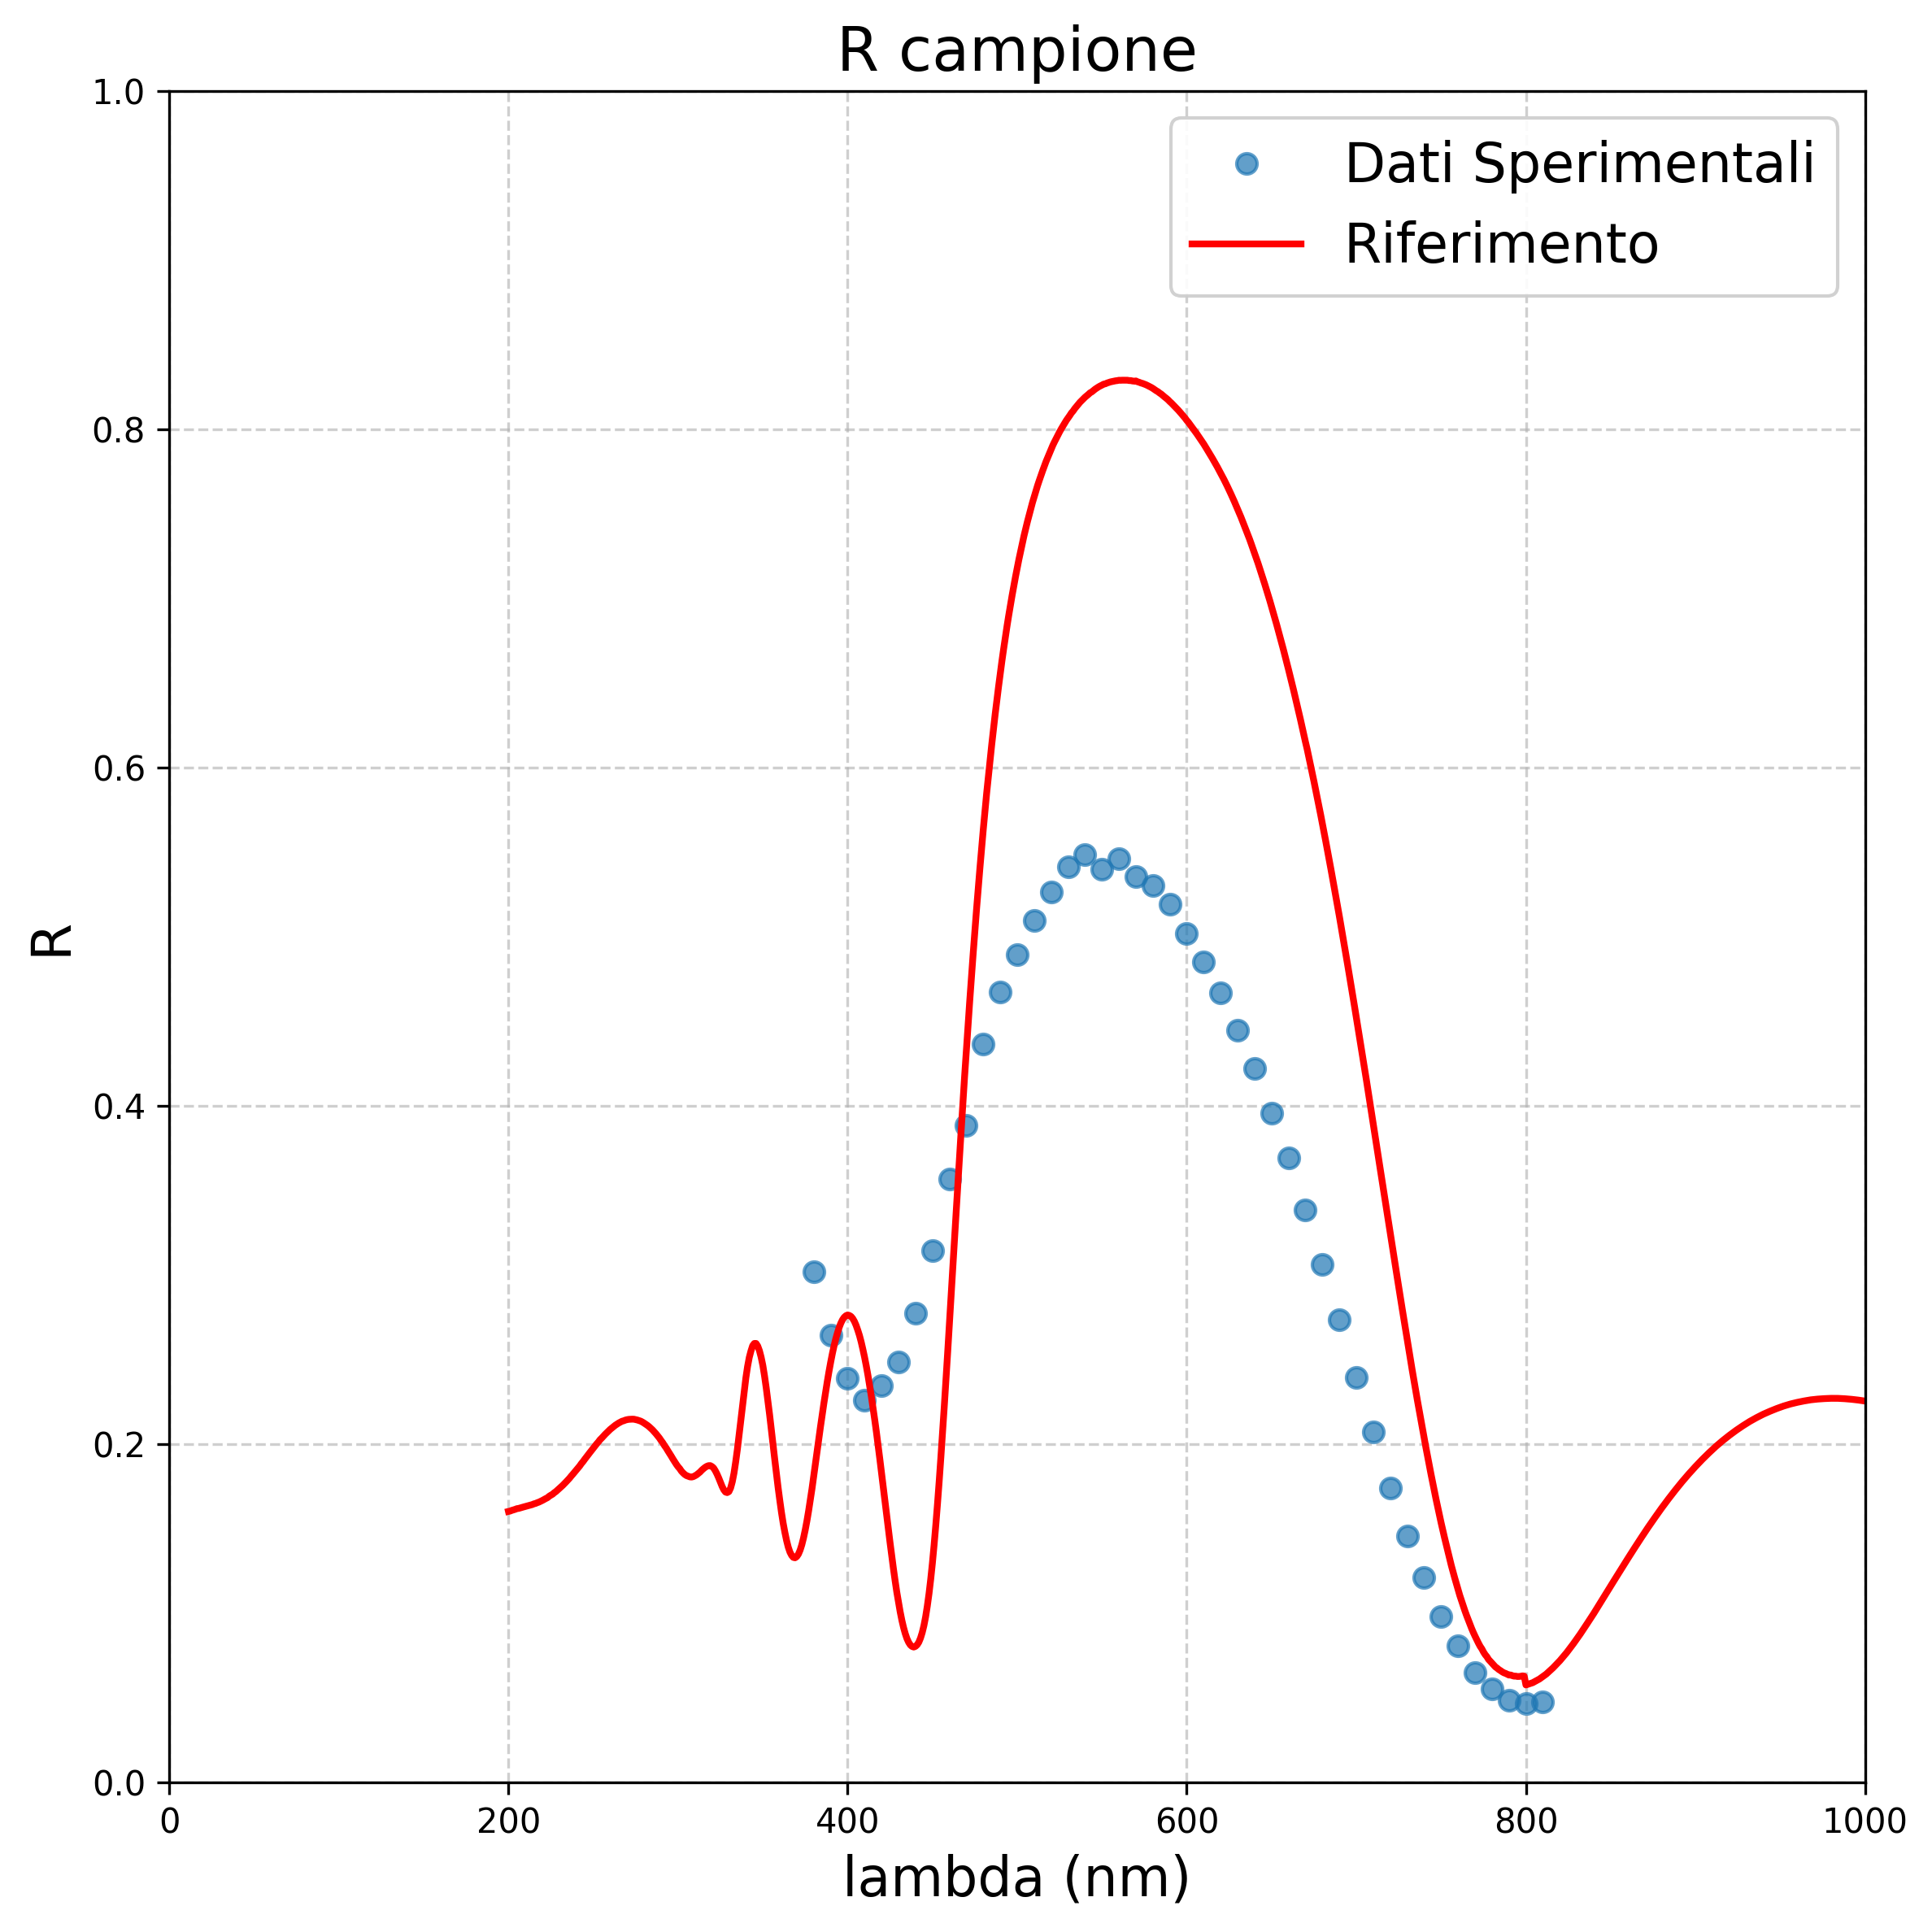
\includegraphics[width=\textwidth]{Confronto_R campione.png}
         \subcaption{Spettro di riflettanza campione n°7}
     \end{subfigure}
\end{figure}
% -------------------------------------------------------------------
\section{Conclusioni}
Gli spettri acquisiti per il vetro amorfo ed il silicio cristallino mostrano un buon accordo con i dati di riferimento ed il comportamento teorico atteso. Tuttavia, nel caso del silicio si osserva un offset sistematico rispetto allo spettro di riferimento. Tale scostamento è probabilmente dovuto ad un lieve disallineamento nell'apparato a causa dell'inclinazione della lastra rispetto al piano del supporto, cosa che ha comportato una parziale attenuazione dell'intensità del segnale.
Invece analizzando la curva di dispersione dell'indice di rifrazione, si osserva come l'andamento sia accuratamente descritto dal modello di Cauchy.
Infine, le misurazioni sul campione incognito mostrano profili coerenti con le curvature di riferimento, evidenziando soprattutto il medesimo effetto filtrante. Anche in questo caso però si rileva un offset nella riflettanza, riconducibile con molta probabilità alla stessa difficoltà di posizionamento del campione nel suo supporto.
\end{document}